\documentclass[twocolumn,11pt]{article}
\setlength{\textheight}{9truein}
\setlength{\topmargin}{-0.9truein}
\setlength{\parindent}{0pt}
\setlength{\parskip}{10pt}
\setlength{\columnsep}{.4in}

\usepackage{amsmath,amsfonts,amssymb,amsthm,bm,caption,calc,ifthen,graphicx,url,hyperref}

\begin{document}
\pagestyle{plain}
\onecolumn
PHYS689 
\newline Homework 7
\newline Will Wainwright
\newline Repository: \href{https://github.com/wjwainwright/PHYS689}{https://github.com/wjwainwright/PHYS689}

\section*{Discussion}
This homework took me a bit to grasp conceptually and longer to implement it in Python. I used Scipy to create a multivariate Gaussian and draw 5000 (x,y) points from that distribution. I then gave these points to the MCMC to fit. The original distribution had a mean of $\mu_x = 1$ and $\mu_y = 9$. After 10000 steps through the MCMC with a proposal width of 0.1, I plotted the results. The posterior distribution has median values of $\mu_x = 1.038045127251182$ and $\mu_y = 8.879400073855749$. The standard deviation on those values is $1.5362625820473927$ and $1.9741523862764494$ respectively. These standard deviations are quite high, partly because of the starting point of (0,0), but also because the MCMC tended to drift around the actual value quite a lot compared to example MCMCs that I have seen. The drifting can be seen in Figure 4. The outcome of the MCMC seems quite variable, and some iterations the median value is farther from the true value than in this case. Regardless, the true value tends to be within a standard deviation of the median, and I would consider that to be a success.

\begin{figure}[!h]
	\centering
	\noindent
	\makebox[\textwidth]{
      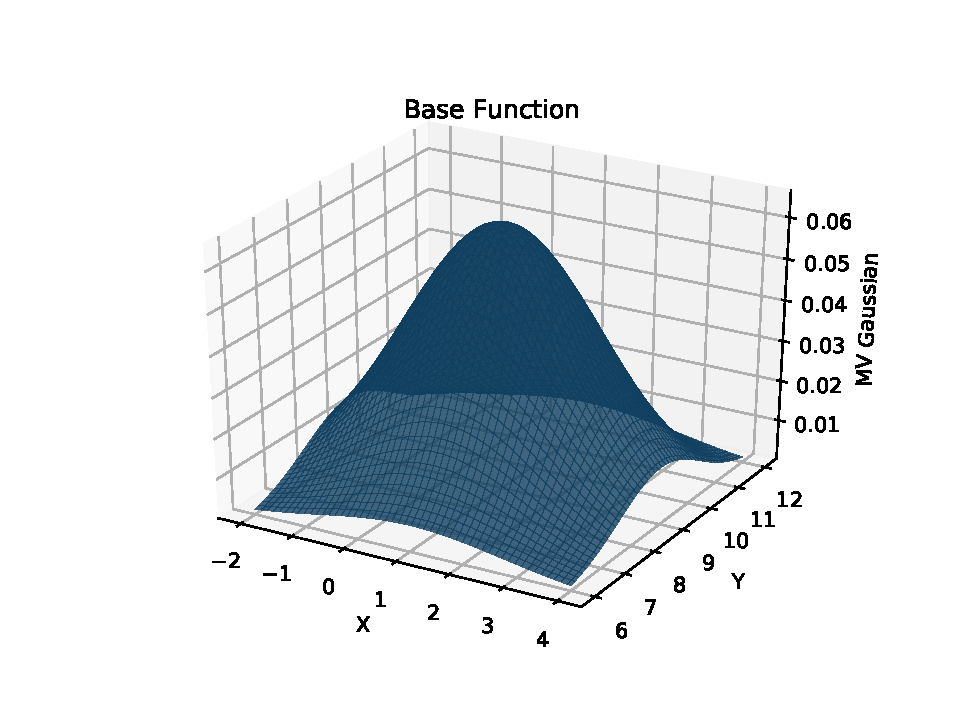
\includegraphics[width=5in]{pdf.pdf}}
      \caption{Base PDF used to generate the random samples in Figure 3. Multivariate Gaussian with a mean of [1,9] and a variance of [3,2].}
\end{figure}

\begin{figure}[!h]
	\centering
	\noindent
	\makebox[\textwidth]{
      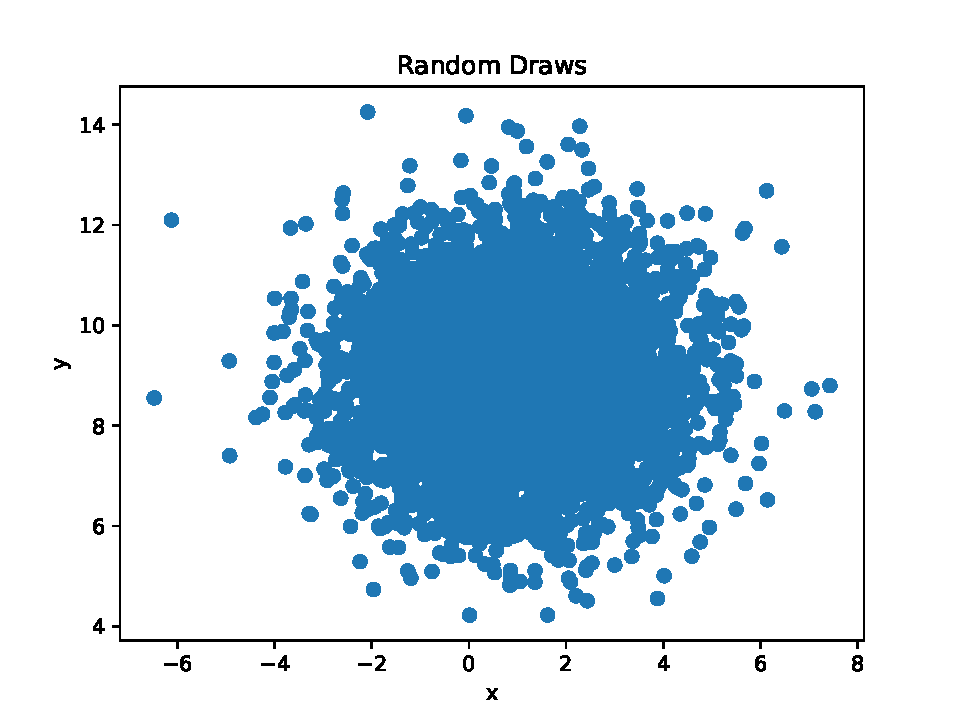
\includegraphics[width=5in]{draws.pdf}}
      \caption{Draws of x \& y from the PDF in Figure 1. These points were used to calculate the likelihood in the MCMC.}
\end{figure}

\begin{figure}[!h]
	\centering
	\noindent
	\makebox[\textwidth]{
      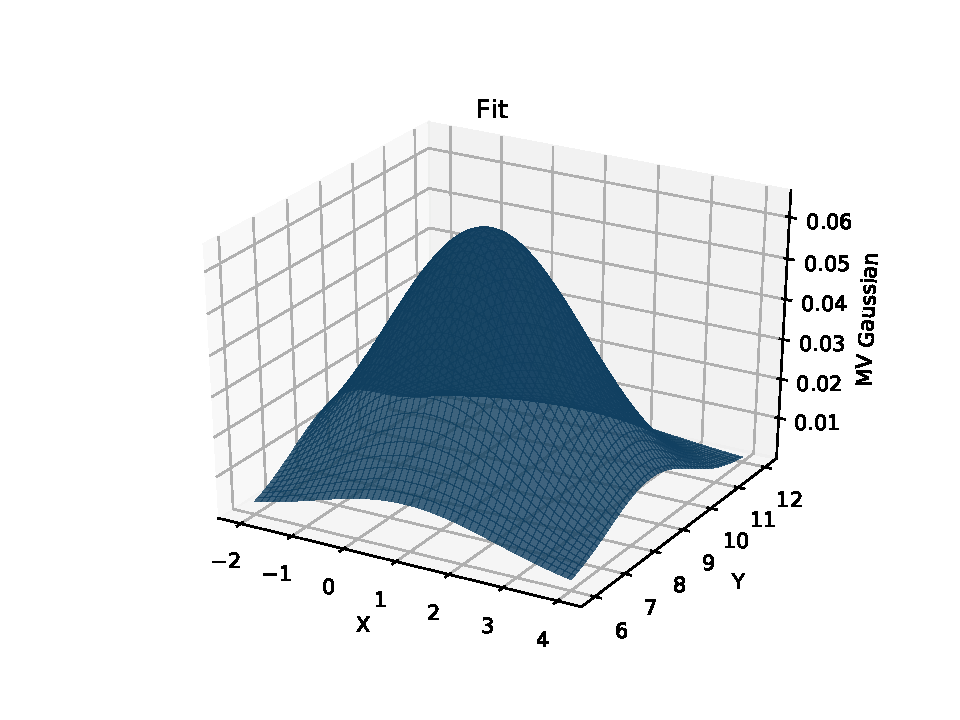
\includegraphics[width=5in]{fit.pdf}}
      \caption{Plot of the fit parameters using the same method used to create Figure 1. The central location of the Gaussian is slightly off compared to in Figure 1.}
\end{figure}


\begin{figure}[!h]
	\centering
	\noindent
	\makebox[\textwidth]{
      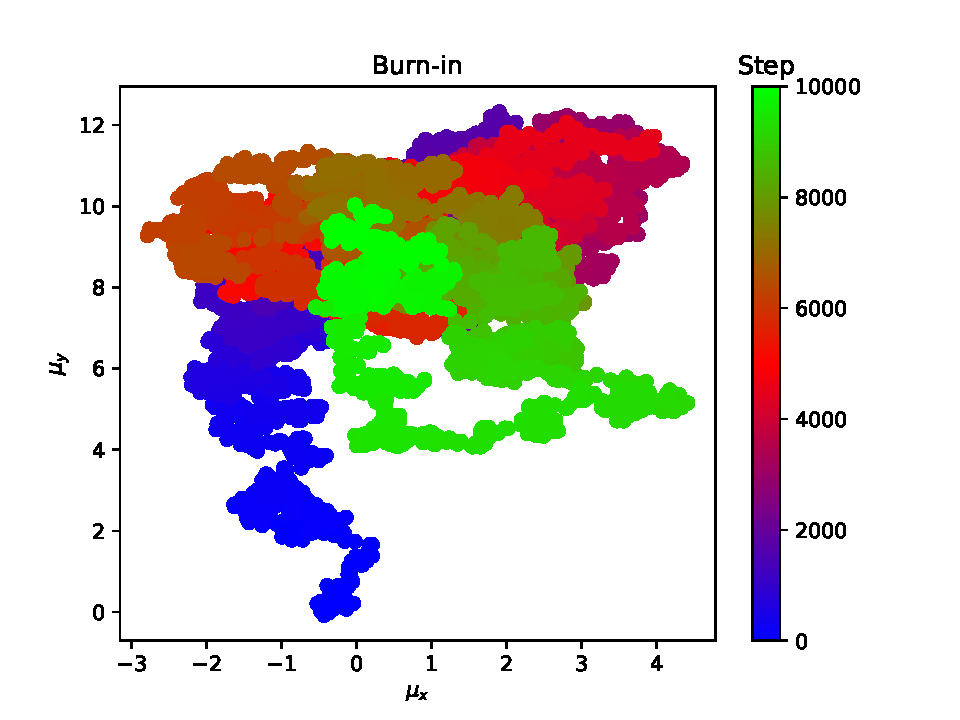
\includegraphics[width=5in]{burn.pdf}}
      \caption{Plot showing the value of $\mu_x$ and $\mu_y$ as a function of the step in the MCMC. The value tends to drift around the actual value of [1,9]. I would say that the burn-in time is at least 2500 samples, but given the variability seen around the true value, I would say 5000 samples are needed to draw a more reliable median or mean that is not as skewed by the first 2000 points.}
\end{figure}



\end{document}